\documentclass[conference]{IEEEtran}
\IEEEoverridecommandlockouts
\usepackage{cite}
\usepackage{graphicx}
\usepackage{placeins}
\usepackage{pifont}
\usepackage{hyperref}
\usepackage{array}
\usepackage{balance}
\usepackage{refstyle}
\usepackage{pgfplots}
\usepackage{bchart}
\setlength{\parindent}{15pt}
\newcolumntype{C}[1]{>{\centering\let\newline\\\arraybackslash\hspace{0pt}}m{#1}}
\usepackage{caption}
\usepackage{amsfonts}
\usepackage[cmex10]{amsmath}


\begin{document}
\title{EyeCloud: A BotCloud Detection System}
\author{
\IEEEauthorblockN{Mohammad Reza Memarian}
\IEEEauthorblockA{University of Padua\\
Padua, Italy\\
\small Email: memarian.m.reza@gmail.com}
\and
\IEEEauthorblockN{Mauro Conti}
\IEEEauthorblockA{University of Padua\\
Padua, Italy\\
\small Email: conti@math.unipd.it}
\thanks{Mauro Conti was supported by Marie Curie Fellowship PCIG11-GA-2012-321980, funded by the European Commission for the PRISM-CODE project. This work has been partially supported by the TENACE PRIN Project 20103P34XC funded by the Italian MIUR, and by the Project "Tackling Mobile Malware with Innovative Machine Learning Techniques" funded by the University of Padua.}
\and
\IEEEauthorblockN{Ville Leppanen}
\IEEEauthorblockA{University of Turku\\
Turku, Finland\\
\small Email: ville.leppanen@utu.fi}

}

\maketitle
\begin{abstract}
Leveraging cloud services, companies and organizations can significantly improve their efficiency, as well as building novel business opportunities. A significant research effort has been put in protecting cloud tenants against external attacks. However, attacks that are originated from elastic, on-demand and legitimate cloud resources should still be considered seriously. The cloud-based botnet or botcloud is one of the prevalent cases of cloud resources misuses. Unfortunately, some of the cloud's essential characteristics enable criminals to form reliable and low cost botclouds in a short time. In this paper, we present EyeCloud, a system that helps to detect distributed infected Virtual Machines (VMs) acting as elements of botclouds. Based on a set of botnet related system level symptoms, EyeCloud groups VMs. Grouping VMs helps to separate infected VMs from others and narrows down the target group under inspection. EyeCloud takes advantages of Virtual Machine Introspection (VMI) and data mining techniques. 
\end{abstract} 

\section{INTRODUCTION}
Cloud computing is a powerful technology for delivering on-demand hosted services in a multi-tenant environment. It enables consumers to have access to a vast amount of computing resources at any desired time. Cloud computing provides suitable infrastructure, for both honest and malicious purposes. On demand self service resources and rapid elasticity are characteristics of cloud computing that create opportunities for cyber criminals to get advantage of cloud resources. As discussed in \cite{ref1}, abuse of cloud services is a prevalent threat to cloud computing. This matter raises the importance of detection and prevention of abuse uses of cloud services for Cloud Service Provider (CSP). A distinctive example of these kind of anomalistic usages of cloud services is formation of botnet in the cloud.

Botnet is a group of infected computer systems that enables a controller to have control over the group. Examples of botnet functions are: DDoS attack, spamming, search engine optimization poisoning, pay-per-click fraud, financial fraud, bitcoin mining and information stealing \cite{ref22}, \cite{ref34}. Botmasters specifically benefit from the cloud's provided infrastructure as cloud computing offers them various possibilities to conduct their desired attacks. In cloud computing, fairly cheap, scalable and reliable resources are always ready for use. So attackers have ready-to-use infrastructure for their malicious activities. Forming a reliable botclould is an easy and low cost procedure while anonymity of criminals can be preserved \cite{ref42}. 

Botnets are moving toward being more elusive that are able to escape detection. Botmasters integrate multiple backup forms of command and control to hide commanding servers. Particularly, DDoS attacks as a consequence of botnets tend to change their attack vectors during a single attack. As described in \cite{ref14}, botnets are becoming more resilient and responding faster to countermeasures, while getting larger in attack volume and frequency of occurrence\cite{ref16}. 

There are various issues that pave the path for criminals to form a botcloud much easier compared to forming a botnet in conventional environments. Some of these issues are: trendiness of large scale diverse attacks \cite{ref36}, cloud specific vulnerabilities \cite{ref9} and some of cloud essential characteristics. Specific features of cloud computing such as image sharing and interest for homogeneity among cloud systems can further ease the formation of botclouds.    

Main botnet detection methods are: honeypot and intrusion detection system (IDS). Using honeypot and applying intrusion detection system on each machine in the cloud are not feasible solutions \cite{ref42} \cite{ref38}. On the other hand, distributed and specific structure of cloud computing requires detection solutions to meet various cloud specific considerations. In order to detect cloud resources misuse, researchers proposed cloud specific detection systems while mostly overlooking prevention capability in their designed systems. Unfortunately, the solutions for detection of botnets in the cloud are not mature yet; in fact attacks using cloud resources are on rise.

In response to challenges above, the BotCloud Detection System (BCDS) needs to: 1) have a broad view over all nodes in the cloud in a cloud-wide manner; 2) be based on cloud core technologies; 3) be reliable for large cloud environments while being effective. 

\textbf{Contribution.}
In this paper we propose EyeCloud, a system that tackles the problem of detecting when infected VMs in a cloud form botclouds. Our EyeCloud adopts new approaches toward data gathering, information correlation and decision making steps. We propose the main correlation module to be placed in an outer level of cloud platform which is the cloud controller. This helps the system to be more practical and have a wider view over the cloud nodes. In data gathering phase, our approach takes advantage of virtualization as one of the cloud core technologies \cite{ref9}. EyeCloud has various detectors in each host that makes the design more reliable. Our result shows that based on the selected attributes, infected VMs that are potential security threats, can be separated from other VMs. 

\textbf{Organization.}
The rest of this paper is organized as follows. Section II gives background information. Section III explains existing approaches for botcloud detection and malware analysis using VMI in the cloud. In Section IV we introduce our novel design for detection of infected systems which can be elements of botclouds, while in Section V we discuss implementation details. In Section VI we discuss and evaluate our results, and in Section VII we explain our conclusion and future research direction.
\section{PRELIMINARY INFORMATION }
In this section, we explain some preliminary information about botcloud, Virtual Machine Monitor (VMM) and Virtual Machine Introspection (VMI).
 
\textbf{BotCloud.}
Botclouds are botnets that are formed based on a CSP's resources. Botcloud misuses cloud's legitimate resources to conduct malicious activities. The program that is responsible for infecting victim's system is called bot. As bots tend to remain hidden, rootkits are used for their activities. Rootkits have some common effects when they infect systems. The collection of these system level effects can be considered as general symptoms.  

\begin{table*}
\centering
\def
\arraystretch{1.2}
\begin{tabular}{|m{4.5cm}|C{1.5cm}|C{0.9cm}|C{1.4cm}|C{1.2cm}|C{1.1cm}|C{1.0cm}|C{0.9cm}|C{1.5cm}|} \hline
System modification & Rustock.B (2006)&Virut (2007)&Koobface (2008)&Tidserv (2008) &Qakbot (2009) &Pilleuz (2009) &Zbot (2010) &Carberp.B (2014) \\ [0.9ex]\hline
File created  & \checkmark &  &\checkmark &\checkmark &\checkmark &\checkmark &\checkmark &\checkmark \\ [0.9ex]\hline
File Deleted  &  &  & &\checkmark &  &\checkmark &  & \\[0.9ex] \hline
File Modified & & \checkmark & &\checkmark &\checkmark &\checkmark & & \\ [0.9ex]\hline
Registry entry created & \checkmark &\checkmark &\checkmark &\checkmark &\checkmark &\checkmark &\checkmark &\checkmark \\ [0.9ex]\hline
Kernel modification & \checkmark &&&&&&&\\ [0.9ex]\hline
Code injection into process/DLL/App & \checkmark &\checkmark &\checkmark &\checkmark &\checkmark &\checkmark &&\\ [0.9ex]\hline\end{tabular}
\begin{center}
\caption{Botnet intended malware functionalities based on \cite{ref20}}
\end{center}
\end{table*}


\textbf{VMM.}
VMM or hypervisor is a software that runs VMs and manages resource allocation to them. The system on which VMM runs is called host. VMMs are either bare-metal or hosted. In case of bare-metal, VMM runs directly on the underlying hardware. In case of hosted, VMM operates on an operating system. There are a variety of commercial and open-source versions of VMMs. One of the open-source VMMs which we also used for our implementation  is Xen. Xen is an open source and widely used VMM. VMs running on Xen are referred as domains. There are two domain types in Xen, privileged domain and unprivileged domain. A supervisor like VM, called Dom0 runs as privileged domain. VMs running on Xen should run either on Hardware-assisted Virtual Machine (HVM) or Para Virtualization (PV) mode. In HVM, VMs are not aware that they are running in a virtualized environment, whereas in PV mode, VMs experience some modification and are aware that they are running on a virtual platform. 


\textbf{VMI.}
VMI is a technique used in virtualization to inspect memory space of a VM from a secure point which can be another VM (i.e., Dom0). This technique is applicable to security monitoring systems which operate within virtual environments. To conduct introspection, an appropriate Application Programming Interface (API) to use is LibVMI \cite{ref11}. LibVMI which currently is usable with XEN and KVM, enables introspecting VM to read from and write to memory of introspected VM. Introspection through VMI is done in an agent-less manner. LibVMI is well integrated with Volatility \cite{ref19}. Volatility is an advanced open source memory forensic framework which offers variety of functions to users for extraction of data from memory snapshots and dumps. As LibVMI has integrity with Volatility, it is possible to use Volatility functions on live VMs while using LibVMI by adding the LibVMI address space to the address space list of Volatility.

\section{RELATED WORK}
In this section, we discuss previous works done on botcloud detection and malware detection in the cloud using VMI.
 
\textbf{Botcloud detection.}
Botclouds are different from conventional botnets in various ways. So detection of them requires some considerations. That is why we mostly focus on previous works done on detection of botclouds instead of botnets in conventional environments. Kebande and Venter \cite{ref3} proposed botnet detection method in the cloud environment using Artificial Immune System (AIS). This mechanism uses a negative selection algorithm. Researchers in \cite{ref41} proposed a botcloud detection method by using principal component analysis. Researchers in \cite{ref4} designed a passive and an active detection module in VMM to look for information in VMs using VMI and profiling bots. Their work mainly focuses on functions in one host and detects infected machines, based on trained node about bot behaviours. They make the botnet profile based on just the API calls done by the applications. 

\textbf{Malware detection in the cloud specifically using VMI.} 
Watson in \cite{ref13} presented a distributed detection system design that combats malware in multi-server cloud. Beidermann and Katzenbeisser in \cite{ref12} presented a research work to detect computer worms in the cloud based on the spreading behaviour. Their solution looks for inconsistencies in behaviour of machines. Researchers in \cite{ref7}, presented tiny VMs called Forensic Virtual Machines (FVMs) to gather information via VMI for detection of malicious activities. Researchers in \cite{ref6} presented a framework for malware detection in the cloud by using symptoms. 

\section{EYECLOUD DESIGN}
In this section, we present our approach toward EyeCloud design. In particular we focus on monitoring (Section IV.A), detection (Section IV.B) and reaction (Section IV.C) methods.  
\subsection{Monitoring method}
Data collectors gather relevant information in wide-spread manner. In our design, we use the concept of FVM for describing data gathering elements \cite{ref7}. As depicted in Figure 1, we assign one FVM per VM to extract system level information from each VM's memory pages at any given time using VMI. Each FVM is dedicated to one VM and looks for existence of all the required symptoms in the VM assigned to it. Assigning one FVM per VM as opposed to one FVM per symptom \cite{ref7}, has various benefits. Introspected VM should only trust to one FVM, which results in monitored VM's Trusted Computing Base (TCB) reduction. In addition, all symptoms are checked at once and frequently instead of random check. FVMs as any VM are not attack resilient. They might get infected too. In time of any FVM infection, other monitored machines can remain immune from consequences of one of the FVM's infection as FVMs do not randomly check other VMs. On the other hand, for deploying the system in large scale, overhead and scalability issues arise. The discussion about mentioned issues are beyond the scope of this paper and requires more algorithm analysis. We will address them in our future work.    

Figure 1 depicts a high level design of EyeCloud with FVMs incorporated in it. FVMs collect data and transfer them to central correlation module. By comparing the EyeCloud design and a typical cloud platform design, cloud controllers can be hosting units for central correlation modules. The reason is because the cloud controller is the outermost entity in a cloud platform design. So, in order to discover distributed attacks on VMs, FVMs do not have to participate in event correlation. This helps to make FVMs lighter. Apart from the method that is used for data collection, determination of what is actually collected is vital. A sample list of symptoms can be defined by determining inconsistencies in an infected VM. We consider Windows operating systems and we focus on system level inconsistencies (i.e., Inconsistencies mentioned in Table I). 

Based on \cite{ref20}, we prepared Table I which depicts common modifications that nine botnet related malware cause to victim's system. Under each malware's name, the year that malware was discovered is mentioned. By looking at Table I, we conclude all the listed malware create registry entries. As a result, creating registry entry is a prevalent action among listed malware. Hence, creation of registry value under a specific key would be a symptom as opposed to the registry entry value. To reduce false positive, one should look for a set of diverse symptoms. So occurrence of number of diverse symptoms among several machines would trigger security alert while revealing differences among VMs.

Based on \cite{ref43}, \cite{ref44}, \cite{ref21}, \cite{ref35} and Table I, a set of inconsistencies that we consider is in the following; \\

1) \textbf{Existence of hidden processes}. Existence of an abnormal process in the process list is rare by advanced malware as their existence will be revealed easily and fast. On the other hand there is an alternative option for malware authors to inject the malicious code into legitimate processes. Hence, relying solely on the name of running processes in the process list is not a  potent method toward detection of malicious software. Another alternative for rootkits, is to unlink the malicious process from the process list's linked list causing the malicious process not to be present in the list of running processes. A process usually is not unlinked from the linked list of processes list, unless there would be possibly malicious activities at the back of it. 

2) \textbf{ Shutting down security mechanisms - Firewall}. In case of Windows operating systems, one of the security mechanisms that can be target of attack is Windows firewall. Windows firewall can be disabled for legitimate purposes too, but appearance of this symptom beside other symptoms in several VMs can be a potentially malicious act.

3) \textbf{Inappropriate commands in history of the command shell}. Adversary may have direct access to the shell of a system and run some commands directly through the shell. One of the use cases for this matter is when adversary has access to the shell and he can install a service through the command line. 

4) \textbf{Existence of hidden DLLs}. Existence of a hidden DLL (unlinked) is another technique that can be used by malicious codes. There is possibility that the DLL is injected into other processes. This possibly requires a new view toward malicious DLL detection. 

5) \textbf{Shutting down security mechanisms - Windows defender}. As we focus on Windows operating system, Windows defender is one of the vital services that should be checked against getting disabled specifically in Windows 7.

6) \textbf{Shutting down security mechanisms - Automatic update}. As updates and patches are necessary for systems to remain secure, automatic updates may be target for being shut down. 

The main audit source location is each VM's memory using VMI technique. Using VM's memory as audit source location has benefit of combating hiding low-level local activities while identifying actual attacking entities. 

Time of detection is in real-time manner. An infected machine is detected to be infected by the correlation element after an actual infection is occurred. The actual infection may not necessarily result as an immediate damage. As the EyeCloud detects malicious VMs based on system symptoms as opposed to behavioural analysis, it can prevent further damages to systems and networks.  
\subsection{Detection method}
EyeCloud's detection logic is based on clustering. Clustering is one of the data mining techniques. Data mining is a wide-spread analytic technique. Clustering is one of the notable branches of data mining that is based on unsupervised learning techniques. Unsupervised learning is finding structures out of unlabelled data sets. 

In EyeCloud's design, we aim to group a set of VMs into subsets such that all elements in each subset group are more similar in comparison to elements in the other group. One group would contain infected VMs while the other would contain clean elements as grouping occurs based on inconsistencies determined earlier. The novelty of the combination of all the solutions is that based on general symptoms and regardless of type of malware, VMs are grouped. So by using a clustering technique, it would be possible to identify a set of VMs that are infected by different malware. 

\begin{figure*}
\begin{center}
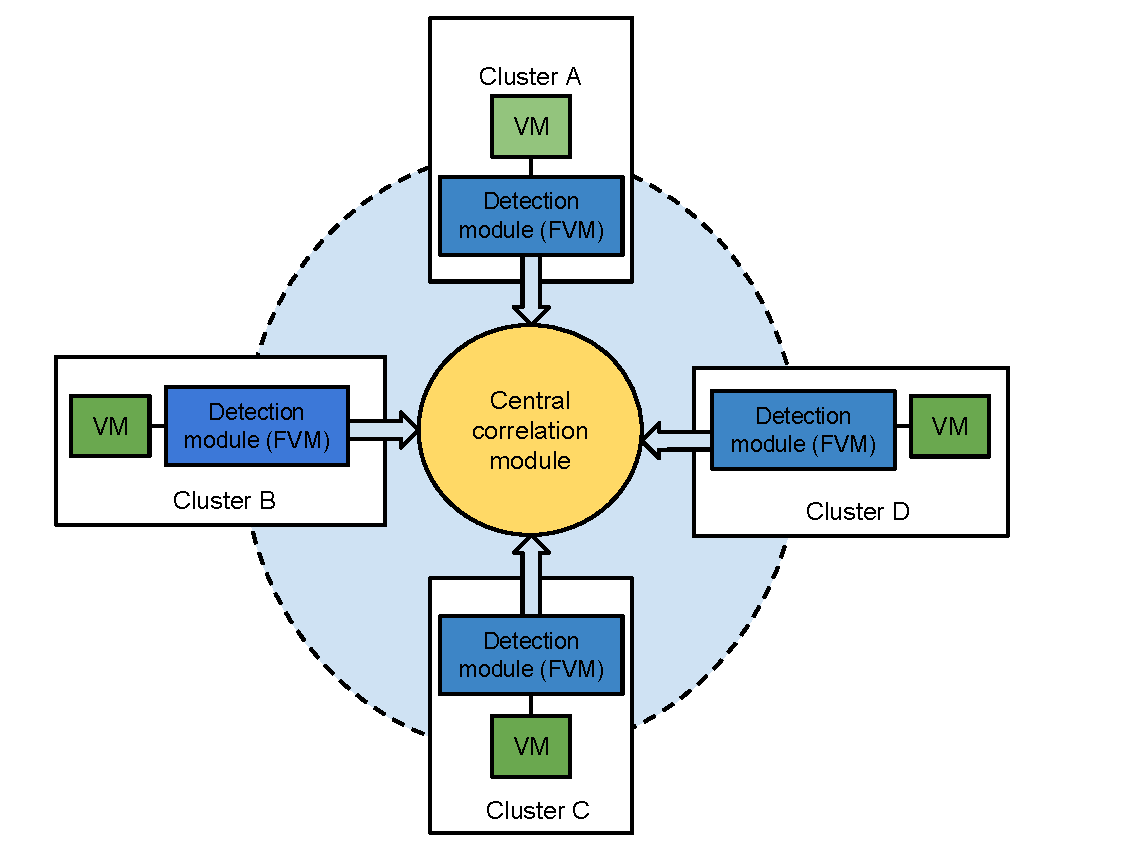
\includegraphics[scale=0.5]{pic111.pdf}
\caption{A wide-spread data collection with central correlation}
\label{Fig:111}
\end{center}
\end{figure*}

Using general symptoms as attributes for clustering algorithm has benefit of reducing signature based technique rules of misuse detection while increasing detection rate. The mentioned technique would increase likelihood of new malware to be detected because system would not need to be updated frequently as signature based systems. On the other hand, there might be false positives too. In our method, likelihood of detection and rate of false positive, heavily depend on the symptoms which are chosen to be checked by detection modules.      

\subsection{Reaction method}
There are two reaction methods that are applicable to the EyeCloud. They are passive and active reaction methods. A passive response does not take correction action against attacking entities. It takes actions such as notifying an administrator. While active response takes corrective actions such as modification of attacking entity. 

EyeCloud has both passive and active response types. Looking at Figure 2, passive method is achieved when analysis and clustering module notifies the alarm and report module about its decision. Administrators are required to analyse the obtained figures and results in this level. Active mode is achieved by the central correlation unit communicating with the VMM of the physical machine holding the infected VM. Central correlation unit can issue a command to the VMM to freeze infected VM's CPU cycle.
\subsection{Infrastructure}
A collaborative detection system consists of several detection elements where each consists of two main components, detection and correlation modules. By getting idea from Software Defined Networking (SDN), we only hold detection modules at the host level in the form of FVMs while having a single main correlation unit. So the EyeCloud can be categorized as a collaborative detection system. 

As depicted in Figure 2, the data collected by each FVM gets in a relevant data structure by symptom search modules. This module only indicate existence or non-existence of symptoms in VMs. The data goes to the central correlation module located in the cloud controller through the VMM. Indeed by placing detective module in the cloud controller level, analytic task gets offloaded from the VMM. As FVMs only collect and pass the data, a separate database is not necessary at their level. A global database is considered in order to communicate with the central correlation unit. Administrators can retrieve different stages of clustering results from the central database.
 
\section{IMPLEMENTATION AND EXPERIMENT}
In this section, we describe our implementation and experiment. In particular, in the first subsection (Section V.A) we describe implementation details. In the second subsection (Section V.B) we explain our experiment details.
\subsection{Implementation}
As for testing the idea that this research is built on it, we set up a test environment. We mainly focus on depicting the possibility of required data collection with desired tools and libraries in order to provide the collected data to clustering algorithm. Furthermore to show that based on the chosen attributes, it is feasible to separate infected VMs from others. 

As the hardware, we used a Dell laptop model Latitude E5440 that consists 8 GB of RAM and an intel core i5 processor. On top of the hardware, we set up a virtualized environment. We used Xen version 4.4 as the VMM. Before setting up Xen, we needed to install an operating system which operates as the Dom0 operating system. Based on experience, Ubuntu 14.04.2 LTS (Linux version 3.16.0-30-generic) was our choice for Dom0. So we set up a Xen 4.4 after we installed an ubuntu 14.04.2. Then we created several VMs running on HVM mode with the Windows 7 professional 32-bit as the operating system. 

As for the introspection tool, we used the LibVMI version 4.4 to conduct introspection. To verify correctness of installation, several examples are provided by the library at time of set up which we ran them to verify correct installation. Next, we configured Volatility framework version 2.4 and connected it to our created live guest VMs. So we used Volatility in conjunction with LibVMI to collect required data by introspecting running VMs. For the sake of acquiring the needed data, we operated data collection from the Dom0 for this experiment.    
\begin{figure}
\hspace{-1.5cm}
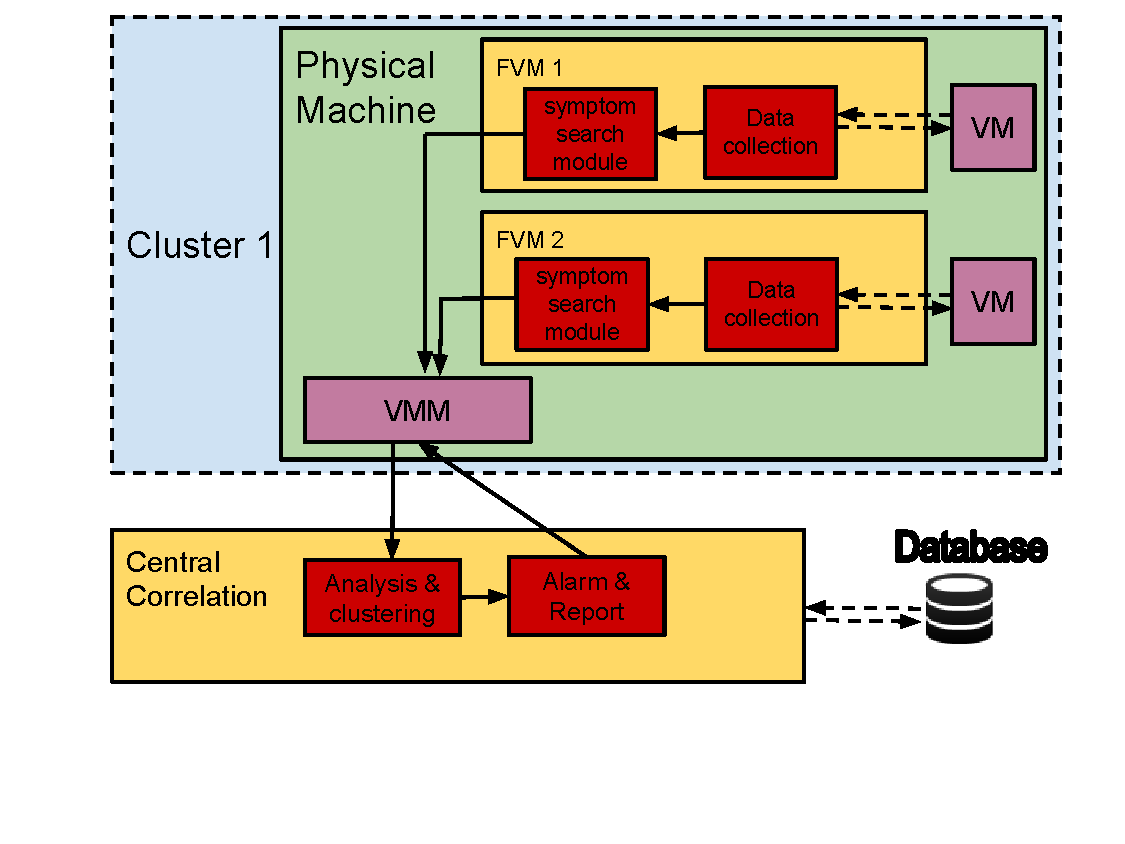
\includegraphics[scale=0.5]{pic114.pdf}
\caption{EyeCloud architecture}
\label{Fig:114}
\end{figure}
\subsection{Experiment}
For a simple illustration of feasibility of our proposed solution and based on our determined inconsistencies (attributes), we considered to collect data using VMI from 13 VMs. Looking at Table II, VM1, VM2, VM3, VM4 and VM5 are considered to be uninfected entities. The mentioned VMs are not infected by any kind of malicious piece of code. Meanwhile various conditions that may happen in non-malicious cases (i.e., shutting down firewall for a legitimate purpose) are considered. For instance we assumed VM2's user to disable one of the security controls of the VM intentionally for legitimate usage.   

As depicted in Table II, we infected VM6 through VM13 with various types of botnet related malware. We chose a sample of Zbot for VM6 and VM7, QAkbot for VM8 and VM9, Koobface for VM10 and VM11 and Pilleuz for VM12 and VM13. So there are pair of VMs infected by the same malware. The first pairs are assumed to have their security controls active, and the second pairs are assumed to have their security controls inactive. We acquired copies of malware that we used from online resources. Accuracy of the obtained malicious files were verified through a legitimate website \cite{ref45}.

For data mining section in the correlation module, we tested the collected data set over the K-means algorithm. For measuring distance between each data point and centroid in the k-means, we used the Euclidean distance algorithm as distance measure. If we assume K (user defined) to be the number of clusters and N to be the number of data points, then in our case, K=2 which is number of groups as well as number of centroids and N=13 (which is number of data points). 

\begin{table*}
\centering
\def
\arraystretch{1.2}
\begin{tabular}{|m{1.2cm}|C{0.8cm}|C{0.8cm}|C{0.8cm}|C{0.8cm}|C{0.8cm}|C{0.8cm}|C{1.5cm}|C{1.0cm}|} \hline
&A.1 &		A.2 & A.3 & A.4 & A.5 & A.6 & Cluster index & Error\\ [1ex]\hline
VM 1 & 		0 & 0 & 0 & 0 & 0 & 0 & 1 & 0.125 \\ [0.9ex]\hline
VM 2 & 		0 & 1 & 0 & 0 & 0 & 0 & 1 & 0.875\\ [0.9ex]\hline
VM 3 & 		0 & 0 & 0 & 0 & 1 & 0 & 1 & 0.875\\ [0.9ex]\hline
VM 4 & 		0 & 0 & 0 & 0 & 0 & 1 & 1 & 0.875\\ [0.9ex]\hline
VM 5 &		0 & 1 & 0 & 0 & 1 & 1 & 2 & 0.72\\ [0.9ex]\hline
VM 6 &		0 & 1 & 0 & 1 & 1 & 1 & 2 & 0.52\\ [0.9ex]\hline
VM 7 &		0 & 0 & 0 & 0 & 0 & 0 & 1 & 0.125\\ [0.9ex]\hline
VM 8 &		1 & 1 & 0 & 1 & 1 & 1 & 2 & 0.32\\ [0.9ex]\hline
VM 9 &		0 & 0 & 0 & 0 & 0 & 0 & 1 & 0.125\\ [0.9ex]\hline
VM 10&		1 &	1 & 0 & 1 & 1 & 1 & 2 & 0.32\\ [0.9ex]\hline
VM 11&		1 & 0 & 0 & 0 & 0 & 0 & 1 & 0.625\\ [0.9ex]\hline
VM 12&		1 & 1 & 0 & 0 & 1 & 1 & 2 & 0.52\\ [0.9ex]\hline
VM 13&		1 & 0 & 0 & 1 & 0 & 0 & 1 & 1.375\\ [0.9ex]\hline

\end{tabular}
\caption{Collected data from VMs using VMI}
\end{table*}

\section{EVALUATION AND DISCUSSION}
In this section, we explain the obtained result of our cluster analysis. As depicted in Table II, each data point is assigned to a cluster. Data points which are grouped in cluster 1, are most of uninfected VMs and infected VMs that had security controls up. Data points that are grouped in cluster 2, are infected VMs that had security controls down. VM5 was not infected and is assigned to cluster 2 which is a false positive. Hence infected VMs that have their security controls off are separated as potential points of threat. This helps to reduce the target group under security analysis. As mentioned previously, result of clustering heavily depends on attributes. In our case attributes are symptoms. 

Result of clustering analysis should be evaluated to measure goodness of clustering analysis. But good results of cluster evaluation does not necessarily depicts a good result for a specific application. A simple evaluation criteria for cluster quality is \textit{Purity}. The maximum value of purity is 1 and the minimum value is 0. Purity result of 1 indicates a perfect clustering. Due to size limit in this paper, we skip the details of purity calculation. The purity of cluster analysis for our system is 0.61 which is higher than average. 

Last column of Table II consists error rates for each data point. Error rate is the distance of a data point from an assigned cluster's centroid. Error rate's occurrences are depicted in Figure 3. As it is shown, 8 data points have error rate of 0.125 or less in this evaluation. Considering false positive points of first group, most of them have high error rate. So they are far from the centroid.    


\section{CONCLUSION AND FUTURE WORK}
Abusing cloud services is a prevalent threat toward cloud computing security. The need for having effective monitoring systems is vital to empower security of the cloud. By making sure about security of the most inner entities of the cloud computing which are VMs, entire security of the cloud can be increased. 

In this paper we presented the EyeCloud, a system which detects members of botnets that abuse cloud resources. Our system takes advantage of data mining and virtual machine introspection techniques to group malicious and non-malicious VMs. By identifying elements of botclouds, further processes can take place on a smaller target group which consists malicious VMs. In this way, analysis can be more accurate and reliable. 

We would like to further investigate the possibilities of applying classification techniques of data mining on the clustered data (malicious VMs cluster). Also expanding the implementation by locating data collection modules in FVMs, testing the proposed solution in a cloud platform and providing methods to protect user's information privacy are our future directions. 
\begin{figure}
\small
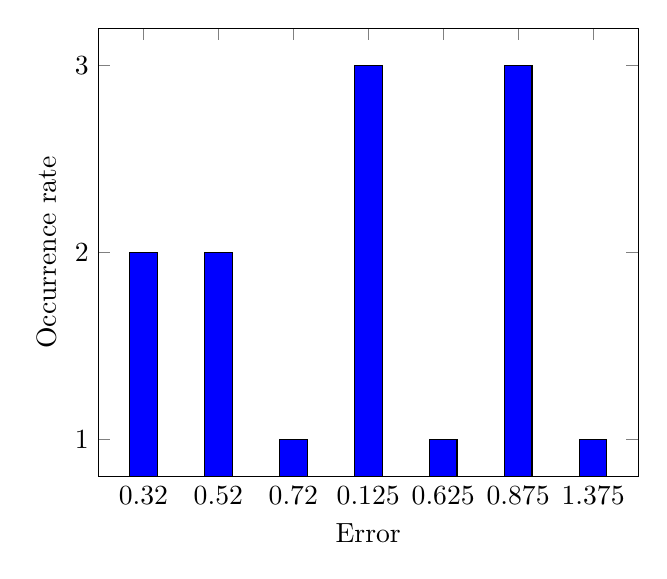
\begin{tikzpicture}
\begin{axis}[
	xlabel=Error,
	ylabel=Occurrence rate,
    symbolic x coords={0.32,0.52,0.72,0.125,0.625,0.875,1.375},
    ytick=data]
    \addplot[ybar,fill=blue] coordinates {
        (0.32, 2)
		(0.52, 2)
		(0.72, 1)
		(0.125, 3)
		(0.625, 1)
		(0.875, 3)
		(1.375, 1)
    };
\end{axis}
\end{tikzpicture}
\begin{center}
\caption{Errors of data points in found clusters}
\end{center}
\end{figure}
\balance

\bibliographystyle{IEEEtran}
\bibliography{ccsref}

\end{document}